\chapter{The Standard Model of particle physics \label{chap:standard_model}}

The Standard Model (SM) of particle physics encapsulates our current understanding of the elementary
particles and their interactions. 
It was developed as a quantum field theory over the past fifty years and has been tested thoroughly
by many different experiments. So far, the Standard Model has proven to be very effective at
predicting and explaining a variety of physics processes. 
In this chapter I will give a short overview of some of the main characteristics of the Standard
Model. For an in-depth and extensive discussion, I refer to
Refs.~\cite{Povh:1995mua,Peskin:1995ev,Burgess:2007zi}.
Section~\ref{sec:SM_particles} will cover the particle content and interactions
present in the Standard Model. The origin of the mass of the elementary particles is touched upon
in Section~\ref{sec:SM_HiggsMechanism}. This chapter concludes with some of the biggest success
stories of the Standard Model in Section~\ref{sec:SM_success}.

\section{Particles and interactions \label{sec:SM_particles}}

The Standard Model contains three families (or generations) of fermionic matter, each consisting of
a charged lepton, a corresponding neutrino, and an up- and down-type quark.
The three charged leptons are the electron ($e$), muon ($\mu$) and tau ($\tau$). Their corresponding
neutrinos are called the electron, muon, and tau neutrino ($\nu_e, \nu_\mu, \nu_\tau$). 
The three quark families comprise the up ($\cPqu$) and down ($\cPqd$) quark, the charm
($\cPqc$) and strange ($\cPqs$) quark, and the top ($\cPqt$) and bottom ($\cPqb$) quark.
Apart from the progressively larger mass of the particles, the three families are exact copies.
Until this day, there is no explanation about why there are three families, and not more or less. 
In fact, the world around us is built solely from particles of the first generation. 
Each atom comprises a nucleus surrounded by electrons. 
The building blocks of the atomic nucleus are the protons and neutrons, which are combinations of up
and down quarks ($\cPqu\cPqu\cPqd$ for the proton and $\cPqu\cPqd\cPqd$ for the neutron).

A theory containing only free particles would be quite uneventfull. The particles would simply
exist.
In Nature there are four fundamental interactions between particles that we currently know of:
gravity, electromagnetism, the weak interaction, and the strong interaction. 
%Only particles carrying the relevant charge can take
%part in the interaction, e.g. the electric charge for electromagnetism. 

The effects of gravity are seen all around us, even though it is by far the weakest of the four
forces. It is the reason the apple falls to the ground, and the planets circle the Sun. 
Gravity is described by general relativity, and is a macroscopic theory that directly affects
everything with a mass. No quantum theory of gravity has been developed yet, although much work has
been done in that direction, and a force carrier, the graviton, has been proposed to exist. For the
energy scales that are probed by particle collisions at the LHC, however, it can be safely ignored,
being too weak to have an effect on the behaviour of the particles involved. 

The remaining three interactions are the ones that are described by the Standard Model of
particle physics. They can be formulated together, as a single, unified, quantum field theory,
governed by the gauge group $SU(3)_c \times SU(2)_L \times U(1)_Y$. The interactions are mediated by
the gauge bosons, which are vector (spin-1) particles. Particles can be charged under each part of
this gauge group, meaning that they feel the corresponding interaction. An overview of the
particles and their charges, the quantum numbers, is given in Table~\ref{tab:SM_particles}. 

The gauge group $SU(3)_c$ describes quantumchromodynamics (QCD). This is commonly referred to as the
strong interaction, the force that binds the quarks inside nucleons. QCD is mediated by the
massless gluons, and affects particles that carry colour charge, of which there are three types:
red (r), green (g) and blue (b). Within the Standard Model only the quarks and gluons carry colour
charge. The strong force has thus no effect on leptons. 
Since the mediators themselves also carry colour charge, this leads to some interesting phenomena,
as discussed in Section~\ref{sec:SM_QCD}. 

The remainder of the SM gauge group, $SU(2)_L \times U(1)_Y$ describes the electroweak interaction. 
The electroweak theory is a chiral theory, which means that left-handed and right-handed particles
transform differently under the gauge group. This is also visible from
Table~\ref{tab:SM_particles}.
The charges of the electroweak interaction are the weak isospin $T_3$, and the hypercharge $Y$. 
The isospin reflects the chiral nature of the theory. Left-handed particles come in doublets, e.g.
the $\cPqu_L$ and $\cPqd_L$ quarks, with weak isospin $\pm 1/2$. Right-handed particles, e.g.
$\cPqu_R$, are singlets under $SU(2)_L$ and have weak isospin 0. 
The mediators are three massless $\W^i$ bosons and a massless $B^0$ boson, respectively. The $\W^i$
bosons form a weak isospin triplet, and the $B^0$ is a weak isospin singlet. 


\begin{table}[t]
  \centering
  \begin{tabular}{ c  c c c  c  r  r  r  c }
    \toprule
    \multirow{2}{*}{Fermions} & \multicolumn{3}{c}{Generation} & \multirow{2}{*}{Spin} &
\multirow{2}{*}{$Q$} & \multirow{2}{*}{$T_3$} & \multirow{2}{*}{$Y$} & \multirow{2}{*}{Colour} \\ 
    & 1 & 2 & 3                      & & & & &  \\ 
    \midrule
    \multirow{4}{*}{Quarks} & \multirow{2}{*}{$\begin{pmatrix} \cPqu \\ \cPqd \end{pmatrix}_L$} 
                            & \multirow{2}{*}{$\begin{pmatrix} \cPqc \\ \cPqs \end{pmatrix}_L$}
                            & \multirow{2}{*}{$\begin{pmatrix} \cPqt \\ \cPqb \end{pmatrix}_L$} 
                            & \multirow{2}{*}{$\frac{1}{2}$} & $+\frac{2}{3}$ & $\frac{1}{2}$ &
\multirow{2}{*}{$\frac{1}{6}$} & \multirow{2}{*}{r,g,b} \\[1ex]
    &  &  &  & & $-\frac{1}{3}$ & $-\frac{1}{2}$ & &   \\
    \cmidrule(lr){2-9}
    & $\cPqu_R$ & $\cPqc_R$ & $\cPqt_R$ & $\frac{1}{2}$ & $+\frac{2}{3}$ & $0$ & $\frac{2}{3}$&
r,g,b \\[1ex]
    & $\cPqd_R$ & $\cPqs_R$ & $\cPqb_R$ & $\frac{1}{2}$ & $-\frac{1}{3}$ & $0$ & $-\frac{1}{3}$ &
r,g,b \\    
    \midrule
    \multirow{3}{*}{Leptons} & \multirow{2}{*}{$\begin{pmatrix} \nu_e \\ e \end{pmatrix}_L$} 
                             & \multirow{2}{*}{$\begin{pmatrix} \nu_\mu \\ \mu \end{pmatrix}_L$} 
                             & \multirow{2}{*}{$\begin{pmatrix} \nu_\tau \\ \tau \end{pmatrix}_L$} 
                             & \multirow{2}{*}{$\frac{1}{2}$} & 0 & $\frac{1}{2}$ &
\multirow{2}{*}{$-\frac{1}{2}$} & \multirow{2}{*}{-}  \\[1ex]
    &  &  &  & & $-1$ & $-\frac{1}{2}$ &  &   \\
    \cmidrule(lr){2-9}
    & $e_R$ & $\mu_R$ & $\tau_R$ & $\frac{1}{2}$ & $-1$ & 0 & $-1$ & - \\
  \bottomrule
  \end{tabular}
  \caption{Overview of all fermions included in the Standard Model, along with the quantum
numbers: electric charge $Q$, third component of weak isospin $T_3$, hypercharge $Y$, and colour.}
  \label{tab:SM_particles}
\end{table}


An important fact is that there cannot be explicit mass terms in the Lagrangian of a chiral theory,
as this would break the gauge symmetry. All particles in the Standard Model should thus be massless.
Of course, this is not what we observe in reality. 
We need a mechanism to introduce masses into our theory without spoiling gauge
invariance. This mechanism is the Brout-Englert-Higgs mechanism, which is based on spontaneous
symmetry breaking, and will be explained in more detail in Section~\ref{sec:SM_HiggsMechanism}.
An important consequence of the symmetry breaking is that the $\W^3$ and $B^0$ bosons mix to
form the photon $\gamma$ and the $\cPZ$ boson. 
The photon remains massless, an indication of the remaining $U(1)_{\text{EM}}$ symmetry,
but the $\W$ and $\cPZ$ bosons acquire mass. 
The conserved charge related to this $U(1)_{\text{EM}}$ symmetry is the electric charge $Q$. We can
express it in terms of weak isospin and hypercharge,
\begin{equation}
  Q = T_3 + Y .
\end{equation}
Electromagnetism can also be described by a quantum field theory: quantumelectrodynamics (QED).
After electroweak symmetry breaking, the $\W^1$ and $\W^2$ are combined into the $\W^+$ and $\W^-$
bosons, which now have a well-defined electric charge. 

Because of this broken symmetry, we observe electromagnetism and the weak force as two distinct
interactions in every day phenomena. 
Because the photon is massless, electromagnetism is a long-range interaction. It describes how
electrically charged particles interact, and is the force that binds atoms and molecules together.
The weak force is mediated by the massive $\W^+$, $\W^-$ and $\cPZ$ bosons.
Heisenberg uncertainty principle dictates that they can thus only exist for a short time. Therefore,
the weak force, which governs radioactive decay, has only a short range.



\section{QCD and asymptotic freedom \label{sec:SM_QCD}}
% confinement
% asymptotic freedom

% probe hadron structure via deep inelastic scattering
% no free quarks ever observed
% How was it possible to describe such a force, strong enough to confine yet weak enough for
% scaling?
% The essential feature of QCD is
% asymptotic freedom [11], according to which its coupling, gs decreases toward short distances and
% increases toward longer distances and times. Asymptotic freedom matches qualitatively with the
% requirements of approximate scaling, and its converse, that the coupling increases toward longer
% distances and times, is consistent with the behavior that gave the strong force its name

The key difference between QCD and QED is that the gluons interact with themselves because they
carry colour charge, unlike the photons, which have no electric charge. The results of this
difference become clear when we consider a given charge at different distance scales. For QED, a
given charge appears smaller the further away the observer is. This property is called
\textit{screening}, and results from the polarization of the vacuum around the charge. 
For QCD the screening effect is also present for quark-antiquark pairs that are created in the
vacuum. However, the gluons that appear also carry colour charge, but with a different polarizing
effect. The further away one goes, the more gluons are visible, and the larger the charge appears.
Conversely, for very short distances, the \textit{antiscreening} effect is much smaller, and the
effective charge is reduced. 

In general, the scaling of a coupling constant in a quantum field theory ($\alpha_S$ for QCD) is
given by the renormalization group equations, and is called the $\beta$-function. For a non-Abelian
quantum field theory like QCD, the $\beta$-function is given by
\begin{equation}
\beta(\alpha_S(\mu)) = \mu^2 \frac{d\alpha_S(\mu)}{d\mu^2} = - (b_0 \alpha_S^2 +  b_1 \alpha_S^3 +
\ldots), 
\label{eq:beta_function}
\end{equation}
with $\mu^2$ the renormalization scale. The one-loop coefficient $b_0$ for QCD with $n_f$ flavours
of quarks is given by
\begin{equation}
  b_0 = \frac{33 - 2n_f}{12\pi}.
\end{equation}
The sign of $b_0$ determines wether the overall theory will exhibit screening or antiscreening. In
our universe, only six quark flavours are known, resulting in a positive value for $b_0$, and an
overall effect of antiscreening. 
It is also clear from Eq.~\ref{eq:beta_function} that a positive $b_0$ means that the size of the
coupling constant diminishes as the momentum scale increases. This is what is called
\textit{asymptotic freedom}. The advantage is that quarks that are very close together can be
treated as free quarks, and that perturbation theory holds. The validity of this picture was
experimentally verified for the first time in deep-inelastic scattering. 
The current world average for the value of the strong coupling constant at the scale of $\cPZ$
boson mass is given by
\begin{equation}
  \alpha_S(M_\cPZ) = 0.1185 \pm 0.0006, 
\end{equation}
and the running of the coupling is shown in Fig.~\ref{fig:running_coupling}. 

\begin{figure}[htpb]
  \centering
  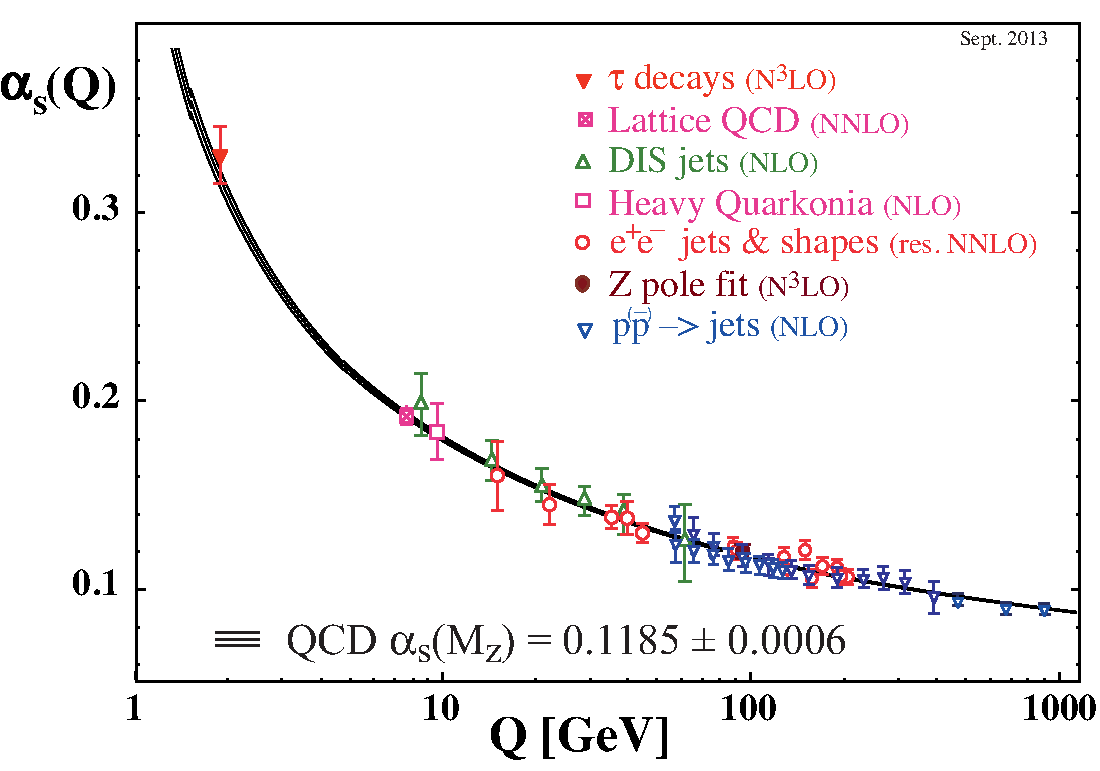
\includegraphics[width=0.8\textwidth]{figures/standardmodel/asq-2013}
  \caption{Latest summary of measurements of $\alpha_S$ as a function of the energy scale $Q$.
The respective degree of QCD perturbation theory used in the extraction of $\alpha_S$ is
indicated in brackets. Figure and caption taken from Ref.~\cite{Agashe:2014kda}
  \label{fig:running_coupling}}
\end{figure}

At very low energy scales, the running of the strong coupling constant results in a very large
value for $\alpha_S$. This explains the observation that no one has ever found a single free quark. 
They are always 'confined' in colorless (white) hadrons, i.e. bound states of quarks and/or
antiquarks.  A quark and antiquark of opposite color (e.g. $r$ and $\overline{r}$) can form a
\textit{meson} and 3 quarks of different color ($r$, $g$ and $b$) can form a \textit{baryon}. 
When one tries to separate two quarks, for example in a high energy collision, they behave like a
string, and energy is built up between them. At some point it becomes energetically more favourable
to use this energy to create extra quarks from the vacuum. 
This process is called hadronization and is responsable for the creation of \textsl{jets}, the
sprays of hadrons that are found at collider experiments. More information on hadronization is
presented in Section~\ref{sec:event_hadronization}.


\section{Brout-Englert-Higgs mechanism \label{sec:SM_HiggsMechanism}}

The Brout-Englert-Higgs mechanism introduces one or more scalar fields, the Higgs
fields, into the theory. These fields acquire a vacuum expectation value that spontaneously
breaks a symmetry in the Lagrangian. 
According to the Goldstone theorem, every spontaneously broken continuous symmetry
results in a massless scalar particle, the Goldstone boson. 
Hence, the number of Goldstone bosons in the theory is equal to the number of broken generators of
the symmetry group. 
However, in the case of a gauge theory, like the Standard Model, this is not the full story. 
We shall see that the massless gauge bosons of the theory acquire a mass by absorbing the Goldstone
boson. 
The number of massive gauge bosons in a spontaneously broken gauge theory will thus be equal to the
number of broken generators. 


Before electroweak symmetry breaking, all four electroweak gauge bosons, $\W^1$, $\W^2$, $\W^3$,
and $B^0$, are massless. What we observe in experiment is one massless gauge boson, the photon
$\gamma$, and three massive gauge bosons ($\W^+, \W^-, \cPZ$). We also know that the electric charge
is conserved. The spontaneous symmetry breaking should thus be of the form
\begin{equation*}
  SU(2)_L \times U(1)_Y \rightarrow U(1)_{\text{EM}} \textrm{ .}
\end{equation*}

For three gauge bosons to acquire mass, three Goldstone bosons will have to be absorbed. As a
consequence, the scalar fields need to contain at least three degrees of freedom for the mechanism
to work. The simplest way to do this is by introducing a complex, scalar $SU(2)$ doublet $\Phi$ with
positive hypercharge ($Y = \frac{1}{2}$)
\begin{equation}
  \Phi = \begin{pmatrix} \phi^+ \\ \phi^0 \end{pmatrix} \textrm{ .} 
\end{equation}
The Standard Model Lagrangian without the strong part, i.e. only the electroweak gauge bosons and
leptons, is given by
\begin{equation}
  \mathcal{L}_{SM} = - \frac{1}{4}W_{\mu\nu}^aW_a^{\mu\nu} - \frac{1}{4}B_{\mu\nu}B^{\mu\nu} +
\overline{L}_i (iD_\mu\gamma^\mu) L_i + \overline{e}_{R,i} (iD_\mu\gamma^\mu) e_{R,i} \textrm{ , } 
\end{equation}
where $i$ runs over the three generations, $\mu,\nu$ are Lorentz indices and $a$ runs over the
number of generators in the gauge group.
The field strengths are given by:
\begin{align*}
  W_{\mu\nu}^a &= \partial_\mu W_\nu^a - \partial_\nu W_\mu^a + g_2 \epsilon^{abc} W_\mu^b W_\nu^c
\\
  B_{\mu\nu} &= \partial_\mu B_\nu - \partial_\nu B_\mu 
\end{align*}
and the covariant derivative for left- and right-handed leptons by:
\begin{align*}
  D_\mu L_L &= \left(\partial_\mu - i g_2 T_a W_\mu^a - i g_1 Y B_\mu \right) L_L \\
  D_\mu e_R &= \left(\partial_\mu - i g_1 Y B_\mu \right) e_R \textrm{ ,}
\end{align*}
where $T_a$ are the generators of the $SU(2)_L$ gauge group and $g_1$, $g_2$ are the coupling
constants for the electroweak interaction.

Now that we have introduced the scalar doublet $\Phi$, we need to add the scalar part to the
Lagrangian
\begin{equation}
  \mathcal{L}_{S} = (D^\mu \Phi)^\dagger(D_\mu \Phi) - V(\Phi), \quad \textrm{with } V(\Phi) = \mu^2
\Phi^\dagger \Phi + \lambda (\Phi^\dagger \Phi)^2 \textrm{ . } 
  \label{eq:scalarlagr}
\end{equation}
The first term is the kinetic term and the second term is the scalar potential, which is often
called the ``Mexican Hat'' potential. The form of the Higgs potential is an assumption in the
Standard Model. It is not known from first principles, but is rather chosen for its nice
properties. 
In order for the vacuum to be stable, the parameter $\lambda$ has to be positive. Depending on the
sign of $\mu^2$ one can distinguish two cases, which are illustrated in
Fig.~\ref{fig:Higgs_potential}. 
In the case $\mu^2 > 0$, the potential $V(\Phi) = \mu^2 \Phi^\dagger \Phi + \lambda (\Phi^\dagger
\Phi)^2$ is always positive with a the minimum  at 
\begin{equation}
\braket{0|\Phi|0} \equiv \Phi_0 = \begin{pmatrix}0\\0\end{pmatrix}. 
\end{equation}
Since the minimum is at the origin, no spontaneous symmetry breaking takes place. 
In case $\mu^2 < 0$, the minimum of the potential is no longer located at the origin. Therefore, the
neutral component of the scalar field can acquire a vacuum expectation value (vev) $v$, thereby
breaking the electroweak symmety.
\begin{equation}
  \braket{0|\Phi|0} \equiv \Phi_0 = \begin{pmatrix} 0 \\ \frac{v}{\sqrt{2}} \end{pmatrix} \textrm{ ,
} \quad v = \sqrt{- \frac{\mu^2}{\lambda}} \textrm{ .}
\end{equation}
By only giving a vev to the neutral component, electromagnetism is conserved, as we set out
to achieve. 

\begin{figure}[htb]
  \centering
  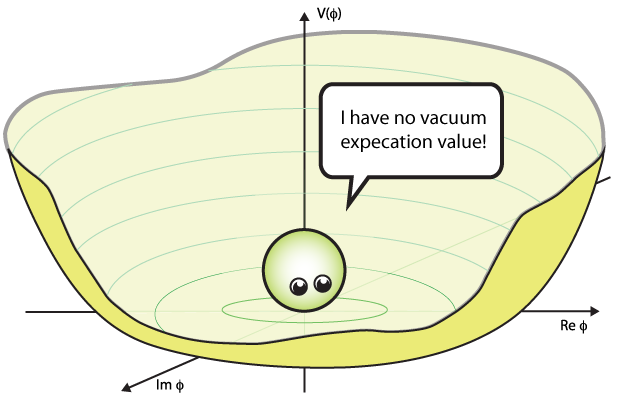
\includegraphics[width=0.48\textwidth]{figures/standardmodel/BoringPotential}
  
  \vspace{2eM}
  
  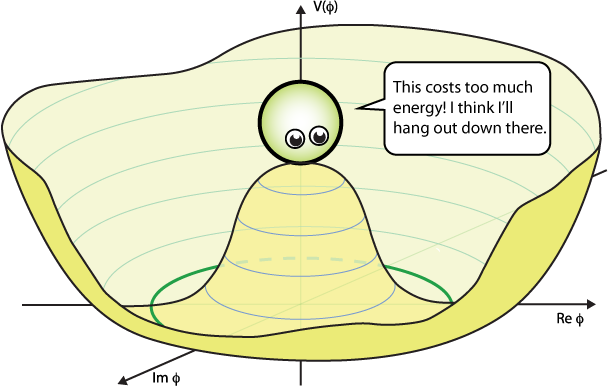
\includegraphics[width=0.48\textwidth]{figures/standardmodel/Higgs-Potential-lookdown}
  ~
  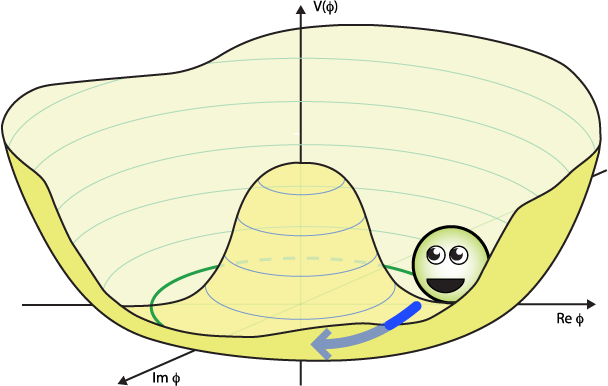
\includegraphics[width=0.48\textwidth]{figures/standardmodel/Higgs-Potential-Goldstone}
  \caption{ [top] The scalar potential with $\mu^2 > 0$ is always positive, with minimum in the
origin. The scalar field will not obtain a vacuum expectation value. 
  [bottom] The scalar potential with $\mu^2 < 0$ has a ``Mexican hat'' shape, with the minimum in a
rim around the origin. The scalar field will thus move from the origin down to the actual minimum
and acquire a vev in the process. The green line indicates a flat direction in the potential,
corresponding to a massless Goldstone mode.
  Figures taken from Ref.~\cite{Higgs_potential}
  \label{fig:Higgs_potential}}
\end{figure}

We proceed by expanding $\Phi$ around its minimum $\Phi_0$
\begin{equation}
  \Phi(x) = \frac{1}{\sqrt{2}} \binom{0}{ v + H(x) } \textrm{ ,}
  \label{eq:higgsexpansion}
\end{equation}
where we have introduced a new scalar field $H(x)$.
After inserting this in the kinetic part of the scalar Lagrangian (Eq.~\ref{eq:scalarlagr}), and
redefining the gauge fields as
\begin{align}
  W^\pm_\mu &= \frac{1}{\sqrt{2}} (W_\mu^1 \mp i W_\mu^2), \\
  Z_\mu &= \frac{1}{\sqrt{g_1^2 + g_2^2}} (g_2W_\mu^3 - g_1 B_\mu),\\
  A_\mu &= \frac{1}{\sqrt{g_1^2 + g_2^2}} (g_2W_\mu^3 + g_1 B_\mu) ,
\end{align}
we find for the kinetic part of the scalar Lagrangian,
\begin{equation}
  |D_\mu \Phi|^2 = \frac{1}{2} (\partial_\mu H)^2 + \frac{1}{2}g_2^2(v+H)^2 W^+_\mu W^{\mu -} +
\frac{1}{8}(v+H)^2 (g_1^2 + g_2^2) Z_\mu Z^\mu \textrm{ .}
\end{equation}
We see that the photon $A_\mu$ remains massless, as required for an unbroken symmetry. Mass terms
for the $W$ and $Z$ bosons have the general form $M_W^2 W_\mu W^\mu$ and $ \frac{1}{2} M_Z^2 Z_\mu
Z^\mu$. We thus find for the gauge boson masses
\begin{align}
  M_W &= \frac{1}{2} v g_2 \\
  M_Z &= \frac{1}{2} v \sqrt{g_1^2 + g_2^2} \\
  M_A &= 0 \textrm{ .}
\end{align}
After spontaneous symmetry breaking, three gauge bosons have thus absorbed a degree of freedom from
the scalars (corresponding to the would-be Goldstone bosons), becoming massive in the process. One
massless gauge boson and one scalar remain.
The remaining scalar degree of freedom $H$ corresponds to the so-called Higgs boson. 

The mixing resulting in orthogonal combinations for the photon and $\cPZ$ bosons is often described
in terms of the Weinberg or weak mixing angle, $\theta_W$,
\begin{align}
  A_\mu &=  \cos \theta_W B_\mu + \sin \theta_W W_\mu^3,\\
  Z_\mu &=  - \sin \theta_W B_\mu + \cos \theta_W W_\mu^3, 
\end{align}
with the Weinberg angle itself defined as
\begin{equation}
  \sin \theta_W = \frac{g_1}{\sqrt{g_1^2 + g_2^2}} .
\end{equation}
At tree level, we also find a relation between the masses of the $\W$ and $\cPZ$ bosons: 
\begin{equation}
  \frac{M_\W}{M_\cPZ} = \frac{g_2}{\sqrt{g_1^2 + g_2^2}} = \cos \theta_W . 
\end{equation}
We will return to this relationship as a way to measure the Weinberg angle in the next section.
Working through the interaction terms between the photon and the fermions, one can show that the
weak mixing angle relates the coupling strength of the weak interaction to that of the
electromagnetic interaction, 
\begin{equation}
  e = g_2 \sin \theta_W .
\end{equation}

The mass and
couplings of the Higgs boson $H$ can be determined from the scalar Lagrangian,
Eq.~\ref{eq:scalarlagr}, upon substituting Eq.~\ref{eq:higgsexpansion}. 
Using $v^2 = -\frac{\mu^2}{\lambda}$ and extracting the parts containing only $H$, we find for the
Lagrangian of the Higgs boson:
\begin{equation}
  \mathcal{L}_H = \frac{1}{2} (\partial_\mu H)(\partial^\mu H) - \lambda v^2 H^2 - \lambda v H^3 -
\frac{\lambda}{4} H^4 \textrm{ .}
\end{equation}
Scalar masses have the general form $\frac{1}{2} m \phi^2$; the Higgs boson mass is thus
\begin{equation}
m_H =  2 \lambda v^2 = - 2 \mu^2,
\end{equation}
and needs to be determined experimentally since there is no other way to access the parameter
$\lambda$. 

Now that we have generated masses for the gauge bosons, all we still need to do, is
generate masses for the fermions as well. This can be done by introducing Yukawa coupling terms
between the fermions and the Higgs fields. 
The Yukawa Lagrangian for the first generation is given by
\begin{equation}
  \mathcal{L}_F = - \lambda_e \overline{L} \Phi e_R - \lambda_d \overline{Q} \Phi d_R - \lambda_u
\overline{Q} \widetilde{\Phi} u_R + h.c. \textrm{ ,}
  \label{eq:Lag_Yuk}
\end{equation}
where we introduced the conjugate of $\Phi$, $\widetilde{\Phi} = i \tau_2 \Phi^*$ which has negative
hypercharge. This is needed to be able to couple to the up-type quarks. It is also possible to
introduce a completely new Higgs doublet with negative hypercharge. This kind of model is called a
two-Higgs doublet model (2HDM) and is needed to introduce supersymmetry (see
Chapter~\ref{chap:supersymmetry}). 

Substituting (\ref{eq:higgsexpansion}) in (\ref{eq:Lag_Yuk}), we find 
\begin{align}
  \mathcal{L}_F &= - \frac{1}{\sqrt{2}} \lambda_e (\overline{\nu}_e, \overline{e}_L) 
		  \begin{pmatrix}0 \\ v+H \end{pmatrix} e_R + ... \\
                &= - \frac{1}{\sqrt{2}} \lambda_e (v+H) \overline{e}_L e_R + ... \textrm{ ,}
  \label{eq:yukawa}
\end{align}
where we highlighted the electron part. 
Fermion mass terms have the general form $m_f \overline{f}_L f_R + h.c.$. We find
\[m_e = \frac{\lambda_e v}{\sqrt{2}} \qquad m_u = \frac{\lambda_u v}{\sqrt{2}} \qquad m_d =
\frac{\lambda_d v}{\sqrt{2}}\]
The neutrinos are seen to remain massless as a result of the lack of a right-handed neutrino in the
Standard Model. 

Using the same doublet of scalar fields we have thus successfully given mass to the gauge bosons and
fermions in our theory. The Brout-Englert-Higgs mechanism also predicts the existence of a massive
scalar particle, the Higgs boson. 
When in 2012 a particle with all the characteristics of this Higgs boson was found at the LHC, this
meant the verification that the process of electroweak symmetry breaking is indeed realized in
nature. 


\section{A success story \label{sec:SM_success}}

Since its conception decades ago, the Standard Model has performed beyond anyone's expectation. 
It has provided an accurate description of results from many accelerator and non-accelerator based
experiments. In this section I will highlight the latest achievement, the discovery of the Higgs
boson, and a global test of the validity of the Standard Model via electroweak precision fits. 

\subsection{Higgs boson discovery}

The existence of the Higgs boson was first proposed in 1964 by Robert Brout and Fran\c{c}ois
Englert, and independently also by Peter Higgs. Nearly half a century later, on the fourth of July,
2012, its discovery was finally announced by the CMS and ATLAS collaboration at the LHC. 
This was a major accomplishment, made possible by the work of thousands of physicists. 

The allowed mass range for the Higgs boson had already been narrowed down by the experiments at LEP
and Tevatron, and by the dataset delivered by the LHC in 2011 at a centre-of-mass energy of 7\TeV. 
In that latter dataset, some evidence for a particle with a mass of around 125\GeV was already
observed, although not strong enough to claim a discovery. 
The energy increase to 8\TeV centre-of-mass energy in 2012 provided just the boost needed to claim
discovery with $5\sigma$ significance. The evidence was strongest in the decay channels
$H\rightarrow\gamma\gamma$ and $H\rightarrow\cPZ\cPZ^*\rightarrow 4\ell$.
Figure~\ref{fig:higgs_discovery} shows the invariant mass distribution of the diphoton and
four-lepton system obtained by the CMS experiment. There is an excess visible around 125\GeV. 
The Higgs boson mass measurement at CMS, combining all decay channels, and combining the 7\TeV and
8\TeV datasets found the following value for the Higgs mass,
\begin{equation}
  m_H = 125.02 {\,}^{+0.26}_{-0.27} (\text{stat}) {\,}^{+0.14}_{-0.15} (\text{syst}) \GeV.
\end{equation}
The measured cross section $\sigma$ also agrees very well with the expectation from the Standard
Model. The signal strength at the measured mass was measured to be
\begin{equation}
 \frac{\sigma}{\sigma_{\text{SM}}} = 1.00 \pm 0.09 (\text{stat}) {\,}^{+0.08}_{-0.07} (\text{theo})
\pm 0.07 (\text{syst})
\end{equation}


\begin{figure}[p]
  \centering
  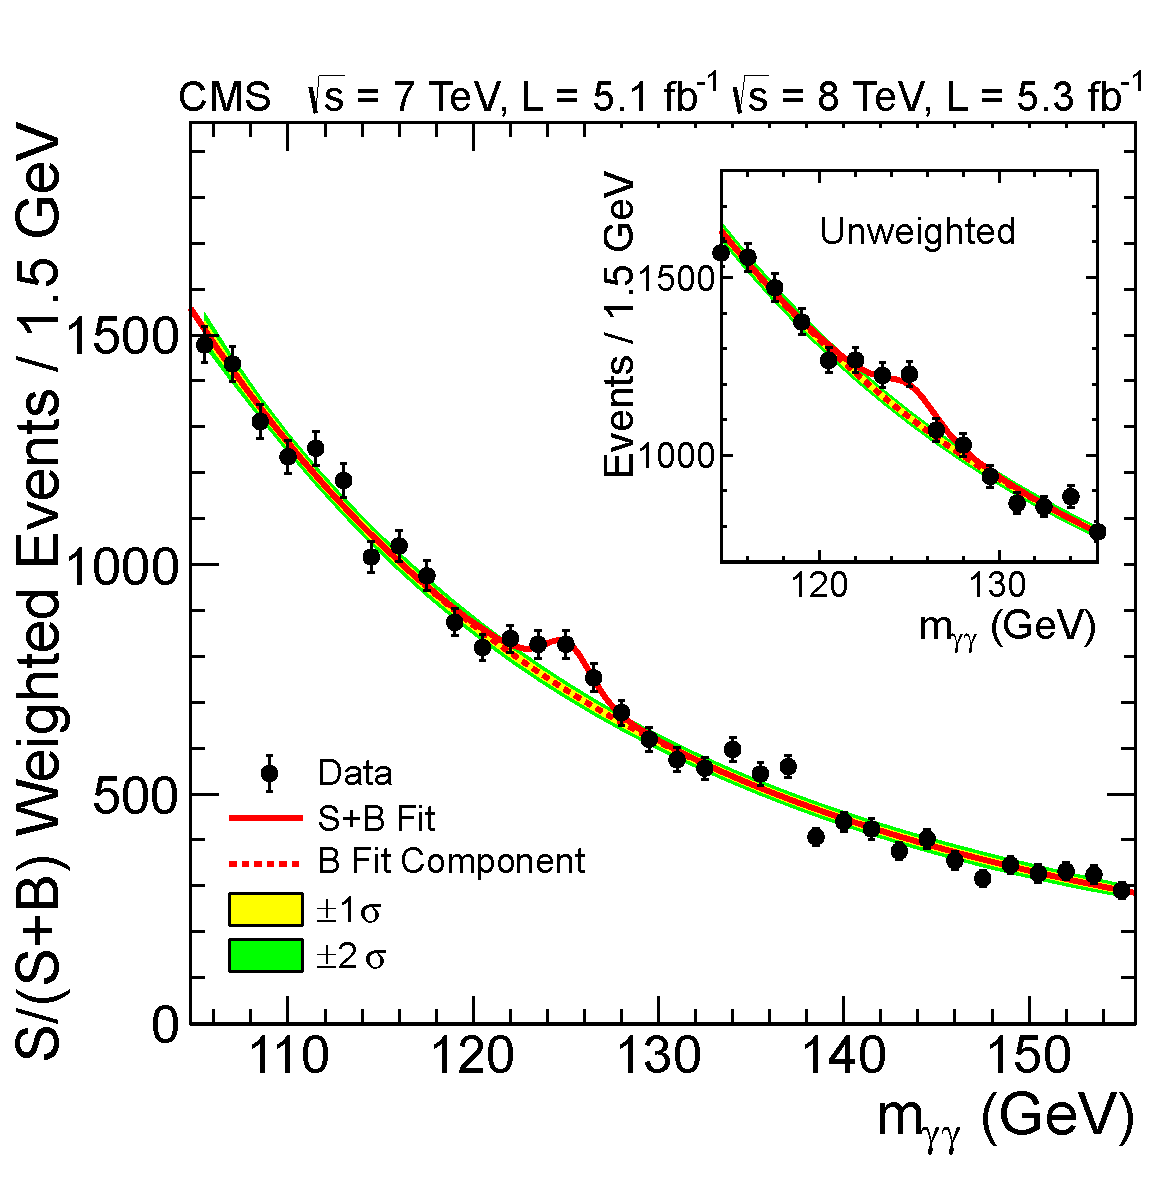
\includegraphics[height=0.29\textheight]{figures/standardmodel/higgs_diphoton}
  ~
  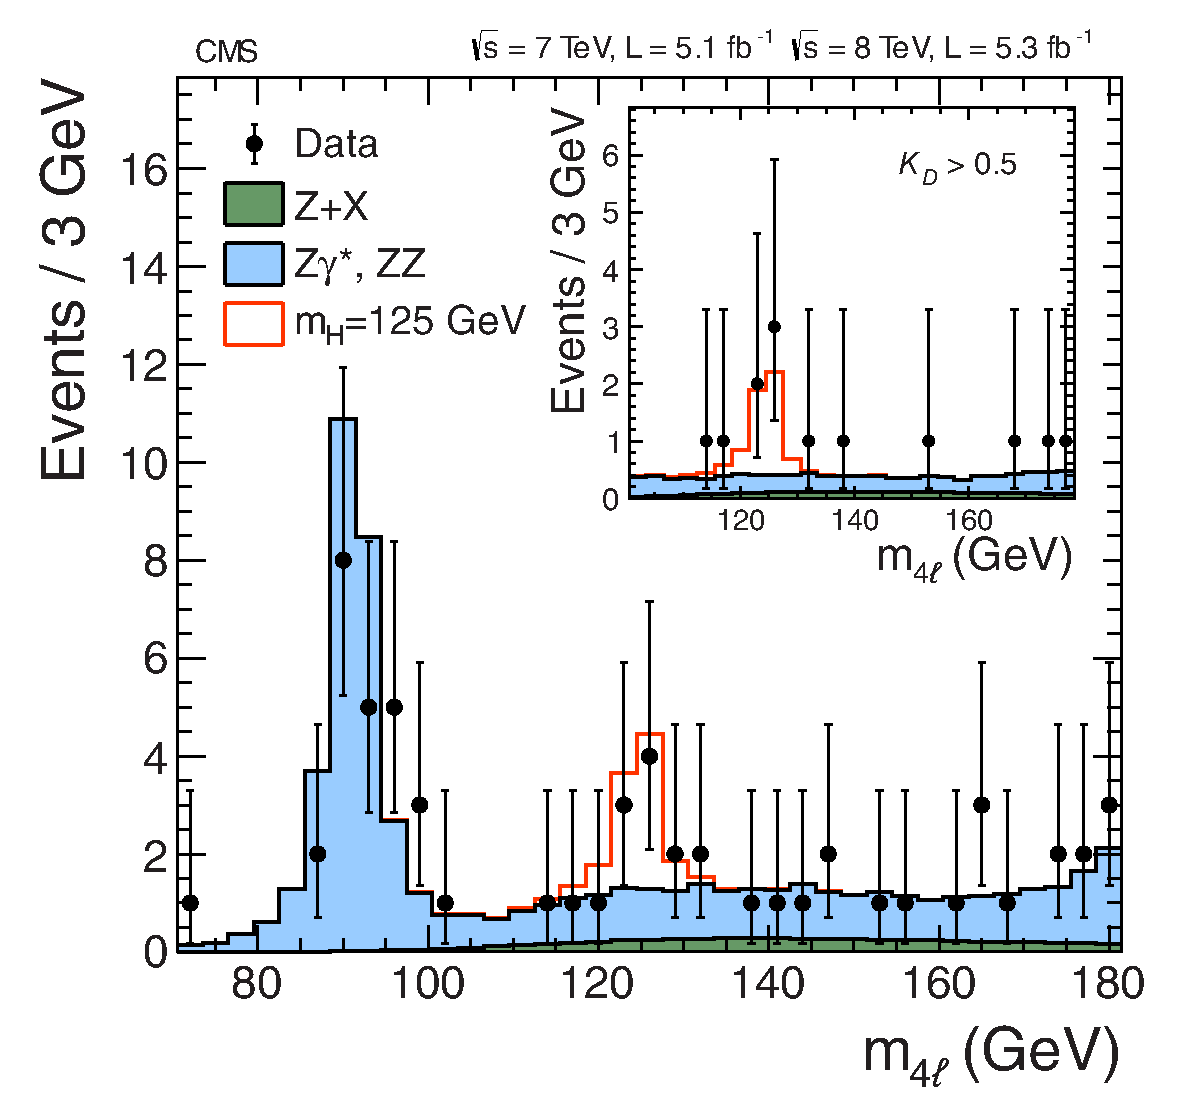
\includegraphics[height=0.28\textheight]{figures/standardmodel/higgs_fourlepton}
  \caption{The Higgs discovery in the two high-resolution channels. Figures taken from
Ref.~\cite{Chatrchyan:2012ufa}.
  [left] The diphoton invariant mass distribution with each event weighted by the
$\frac{S}{S+B}$ value of its category. The lines represent the fitted background and signal, and
the coloured bands represent the ±1 and ±2 standard deviation uncertainties in the background
estimate. 
  [right] Distribution of the four-lepton invariant mass for the $\cPZ\cPZ \rightarrow 4\ell$
analysis. The points represent the data, the filled histograms represent the background, and the
open histogram shows the signal expectation for a Higgs boson of mass $m_H = 125\GeV$, added to the
background expectation.
  \label{fig:higgs_discovery}}
\end{figure}

\begin{figure}[p]
  \centering
  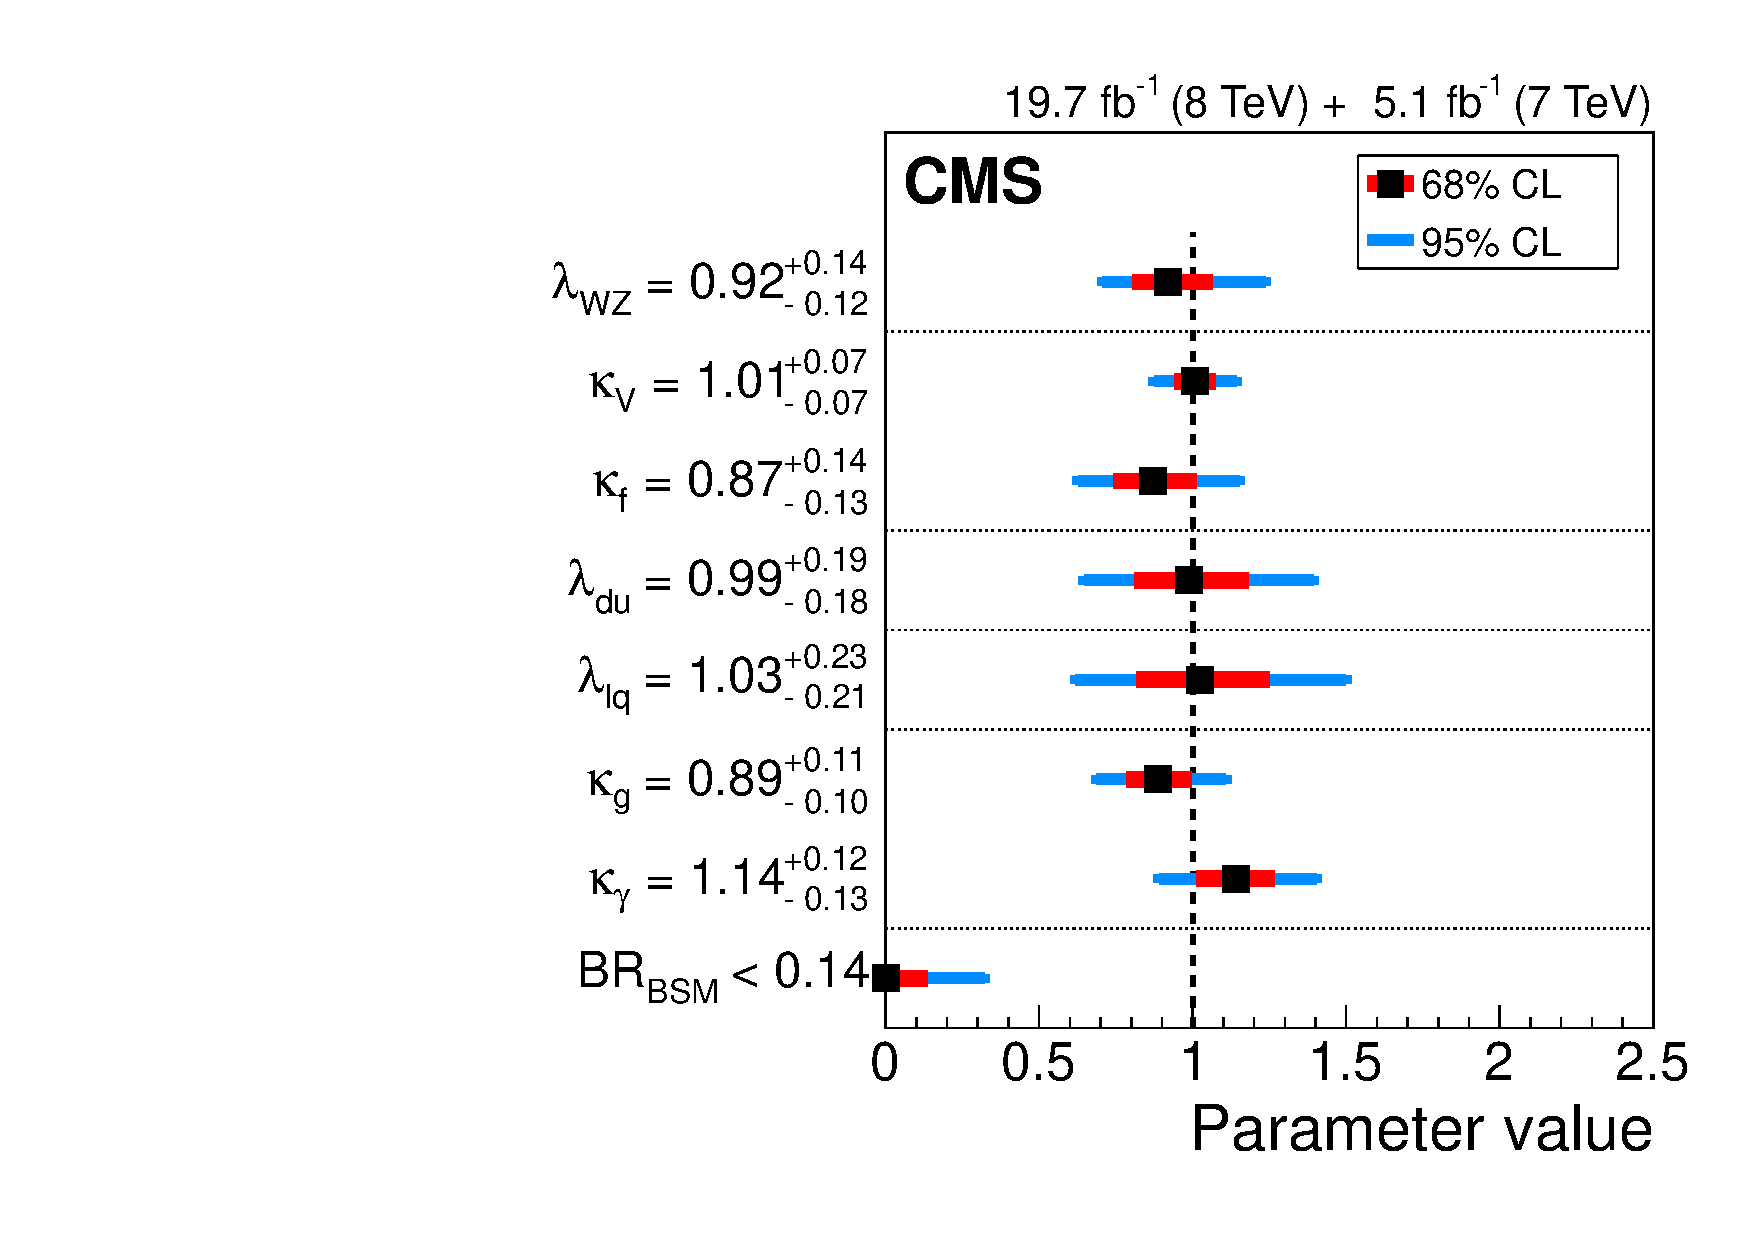
\includegraphics[width=0.7\textwidth]{figures/standardmodel/sqr_summary_lhcxswg}
  \caption{ Summary of tests of the compatibility of the CMS data with the SM Higgs boson
couplings. The observed boson is fully compatible with the Standard Model expectation. Figure taken
from Ref.~\cite{Khachatryan:2014jba}.
  \label{fig:higgs_sm_test}}
\end{figure}


\subsection{Precision electroweak fits}


\begin{figure}[p]
\begin{minipage}{0.44\textwidth}
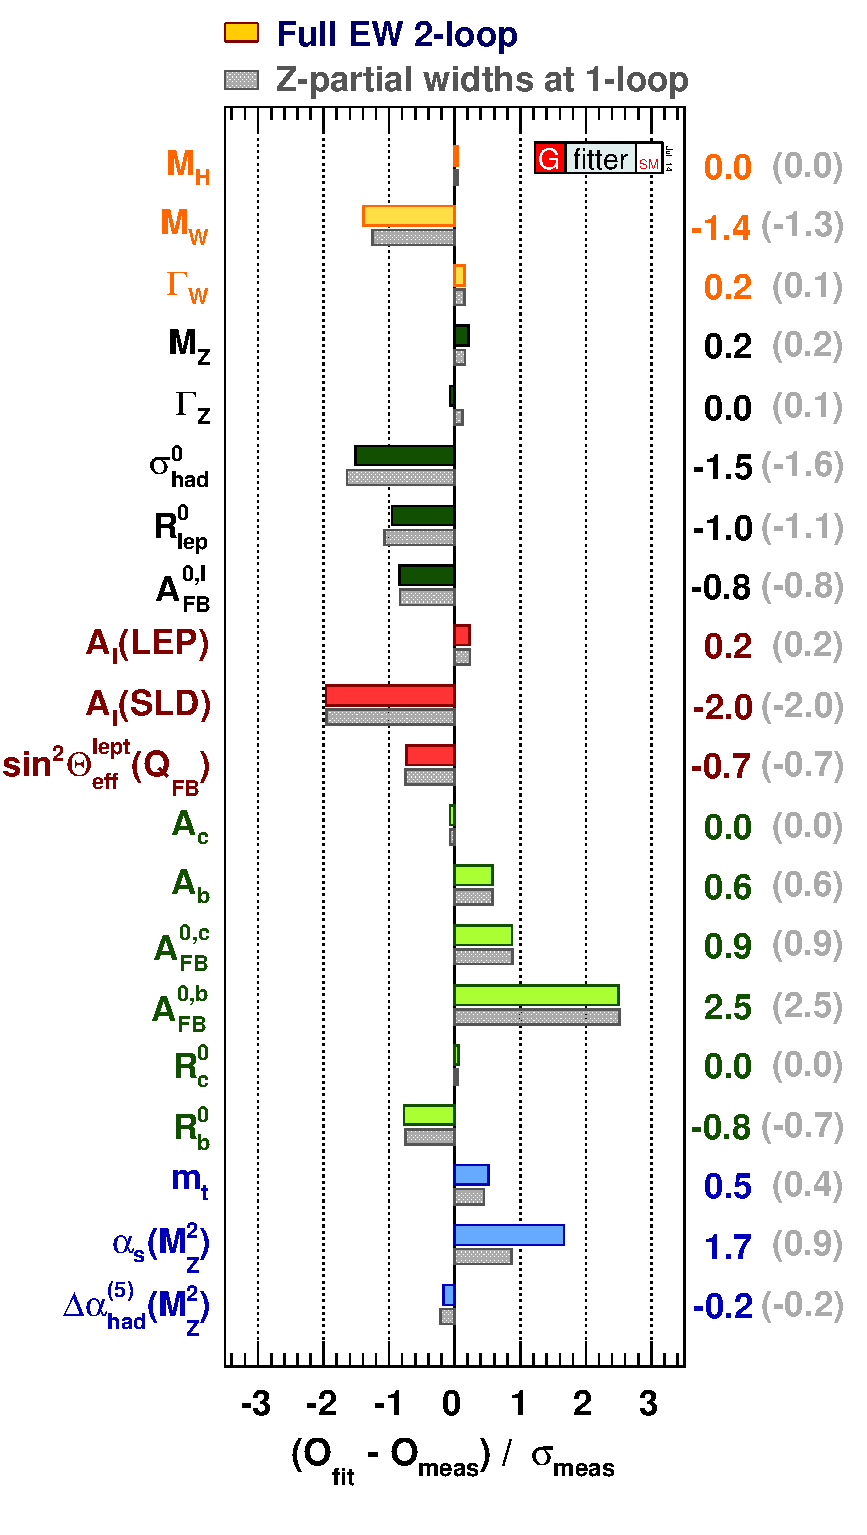
\includegraphics[width=\textwidth]{figures/standardmodel/2014_07_16_PullPlotTwoBarsTwoTheos_logo}
\end{minipage}
\hfill
\begin{minipage}{0.54\textwidth}
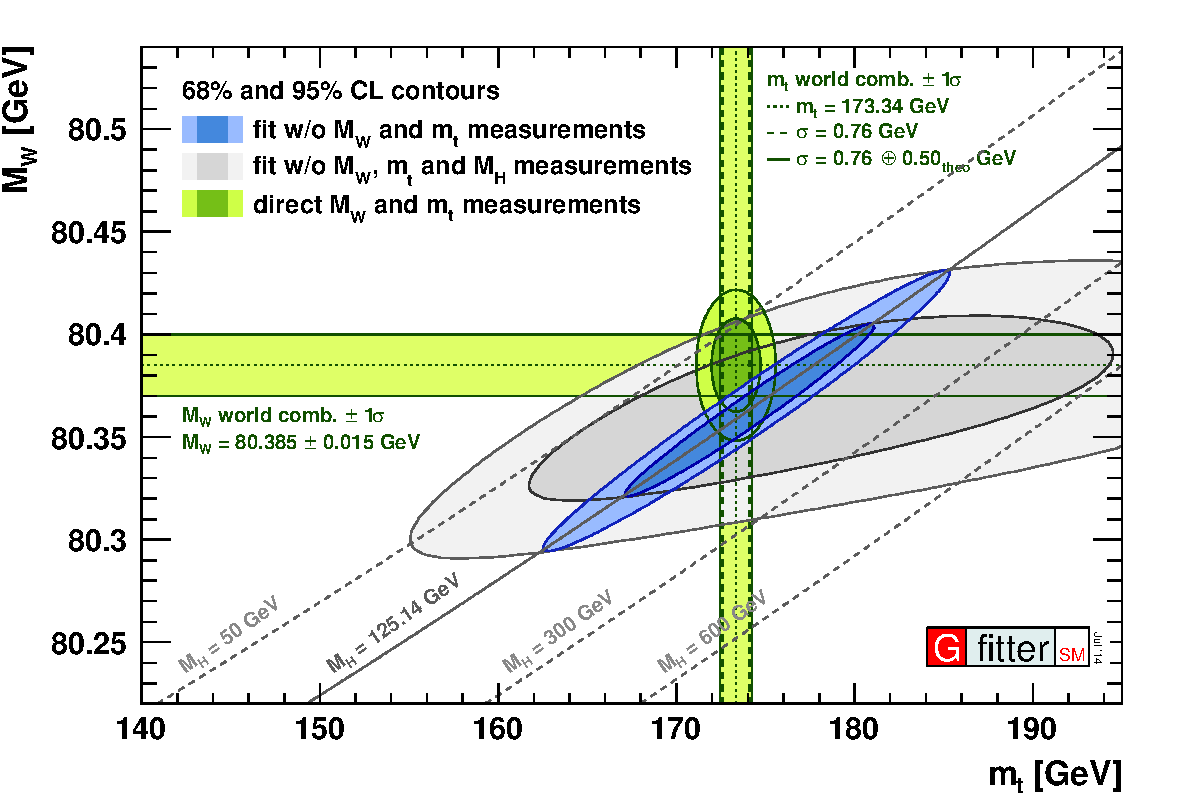
\includegraphics[width=\textwidth]{figures/standardmodel/2014_07_16_Scan2D_MWvsmt_logo}
 
 \vspace{1eM}
 
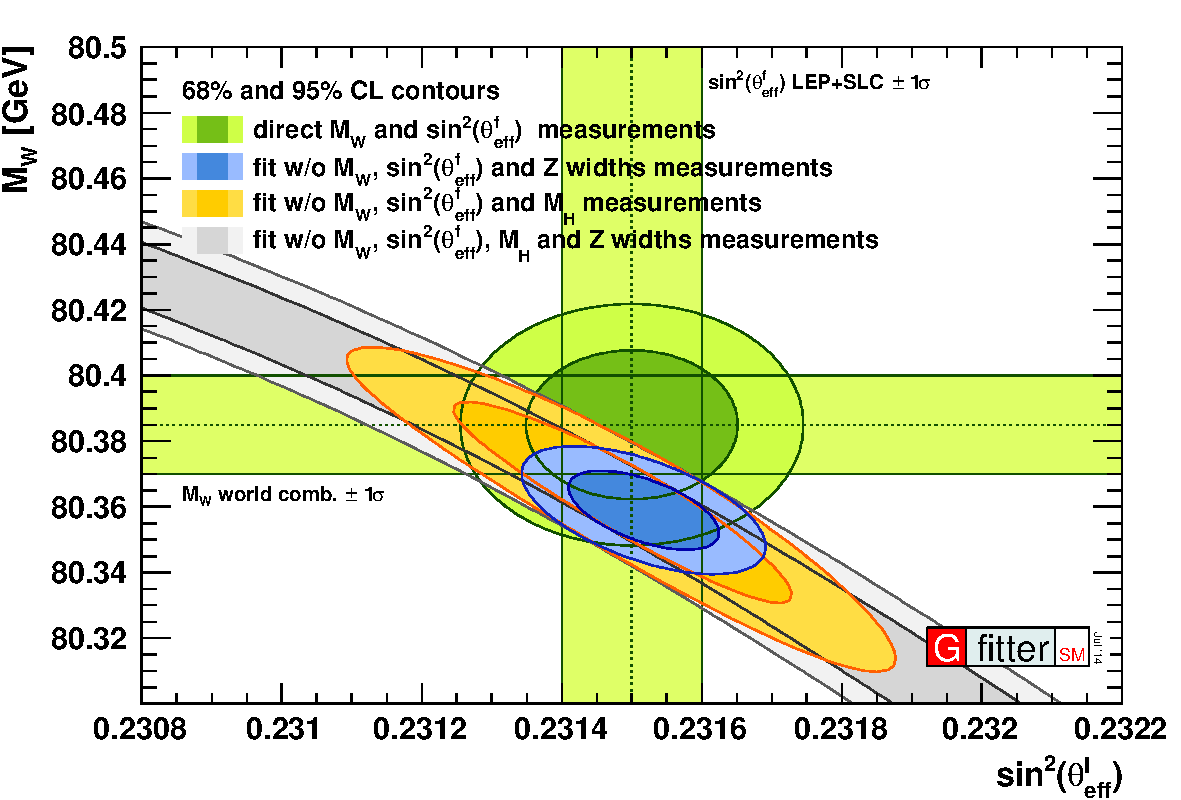
\includegraphics[width=\textwidth]{figures/standardmodel/2014_07_16_Scan2D_MWvsSinEffLep_logo}
\end{minipage}
\caption{ \cite{Baak:2014ora}
\label{fig:global_fit}}
\end{figure}



